\documentclass[1p]{elsarticle_modified}
%\bibliographystyle{elsarticle-num}

%\usepackage[colorlinks]{hyperref}
%\usepackage{abbrmath_seonhwa} %\Abb, \Ascr, \Acal ,\Abf, \Afrak
\usepackage{amsfonts}
\usepackage{amssymb}
\usepackage{amsmath}
\usepackage{amsthm}
\usepackage{scalefnt}
\usepackage{amsbsy}
\usepackage{kotex}
\usepackage{caption}
\usepackage{subfig}
\usepackage{color}
\usepackage{graphicx}
\usepackage{xcolor} %% white, black, red, green, blue, cyan, magenta, yellow
\usepackage{float}
\usepackage{setspace}
\usepackage{hyperref}

\usepackage{tikz}
\usetikzlibrary{arrows}

\usepackage{multirow}
\usepackage{array} % fixed length table
\usepackage{hhline}

%%%%%%%%%%%%%%%%%%%%%
\makeatletter
\renewcommand*\env@matrix[1][\arraystretch]{%
	\edef\arraystretch{#1}%
	\hskip -\arraycolsep
	\let\@ifnextchar\new@ifnextchar
	\array{*\c@MaxMatrixCols c}}
\makeatother %https://tex.stackexchange.com/questions/14071/how-can-i-increase-the-line-spacing-in-a-matrix
%%%%%%%%%%%%%%%

\usepackage[normalem]{ulem}

\newcommand{\msout}[1]{\ifmmode\text{\sout{\ensuremath{#1}}}\else\sout{#1}\fi}
%SOURCE: \msout is \stkout macro in https://tex.stackexchange.com/questions/20609/strikeout-in-math-mode

\newcommand{\cancel}[1]{
	\ifmmode
	{\color{red}\msout{#1}}
	\else
	{\color{red}\sout{#1}}
	\fi
}

\newcommand{\add}[1]{
	{\color{blue}\uwave{#1}}
}

\newcommand{\replace}[2]{
	\ifmmode
	{\color{red}\msout{#1}}{\color{blue}\uwave{#2}}
	\else
	{\color{red}\sout{#1}}{\color{blue}\uwave{#2}}
	\fi
}

\newcommand{\Sol}{\mathcal{S}} %segment
\newcommand{\D}{D} %diagram
\newcommand{\A}{\mathcal{A}} %arc


%%%%%%%%%%%%%%%%%%%%%%%%%%%%%5 test

\def\sl{\operatorname{\textup{SL}}(2,\Cbb)}
\def\psl{\operatorname{\textup{PSL}}(2,\Cbb)}
\def\quan{\mkern 1mu \triangleright \mkern 1mu}

\theoremstyle{definition}
\newtheorem{thm}{Theorem}[section]
\newtheorem{prop}[thm]{Proposition}
\newtheorem{lem}[thm]{Lemma}
\newtheorem{ques}[thm]{Question}
\newtheorem{cor}[thm]{Corollary}
\newtheorem{defn}[thm]{Definition}
\newtheorem{exam}[thm]{Example}
\newtheorem{rmk}[thm]{Remark}
\newtheorem{alg}[thm]{Algorithm}

\newcommand{\I}{\sqrt{-1}}
\begin{document}

%\begin{frontmatter}
%
%\title{Boundary parabolic representations of knots up to 8 crossings}
%
%%% Group authors per affiliation:
%\author{Yunhi Cho} 
%\address{Department of Mathematics, University of Seoul, Seoul, Korea}
%\ead{yhcho@uos.ac.kr}
%
%
%\author{Seonhwa Kim} %\fnref{s_kim}}
%\address{Center for Geometry and Physics, Institute for Basic Science, Pohang, 37673, Korea}
%\ead{ryeona17@ibs.re.kr}
%
%\author{Hyuk Kim}
%\address{Department of Mathematical Sciences, Seoul National University, Seoul 08826, Korea}
%\ead{hyukkim@snu.ac.kr}
%
%\author{Seokbeom Yoon}
%\address{Department of Mathematical Sciences, Seoul National University, Seoul, 08826,  Korea}
%\ead{sbyoon15@snu.ac.kr}
%
%\begin{abstract}
%We find all boundary parabolic representation of knots up to 8 crossings.
%
%\end{abstract}
%\begin{keyword}
%    \MSC[2010] 57M25 
%\end{keyword}
%
%\end{frontmatter}

%\linenumbers
%\tableofcontents
%
\newcommand\colored[1]{\textcolor{white}{\rule[-0.35ex]{0.8em}{1.4ex}}\kern-0.8em\color{red} #1}%
%\newcommand\colored[1]{\textcolor{white}{ #1}\kern-2.17ex	\textcolor{white}{ #1}\kern-1.81ex	\textcolor{white}{ #1}\kern-2.15ex\color{red}#1	}

{\Large $\underline{12n_{0282}~(K12n_{0282})}$}

\setlength{\tabcolsep}{10pt}
\renewcommand{\arraystretch}{1.6}
\vspace{1cm}\begin{tabular}{m{100pt}>{\centering\arraybackslash}m{274pt}}
\multirow{5}{120pt}{
	\centering
	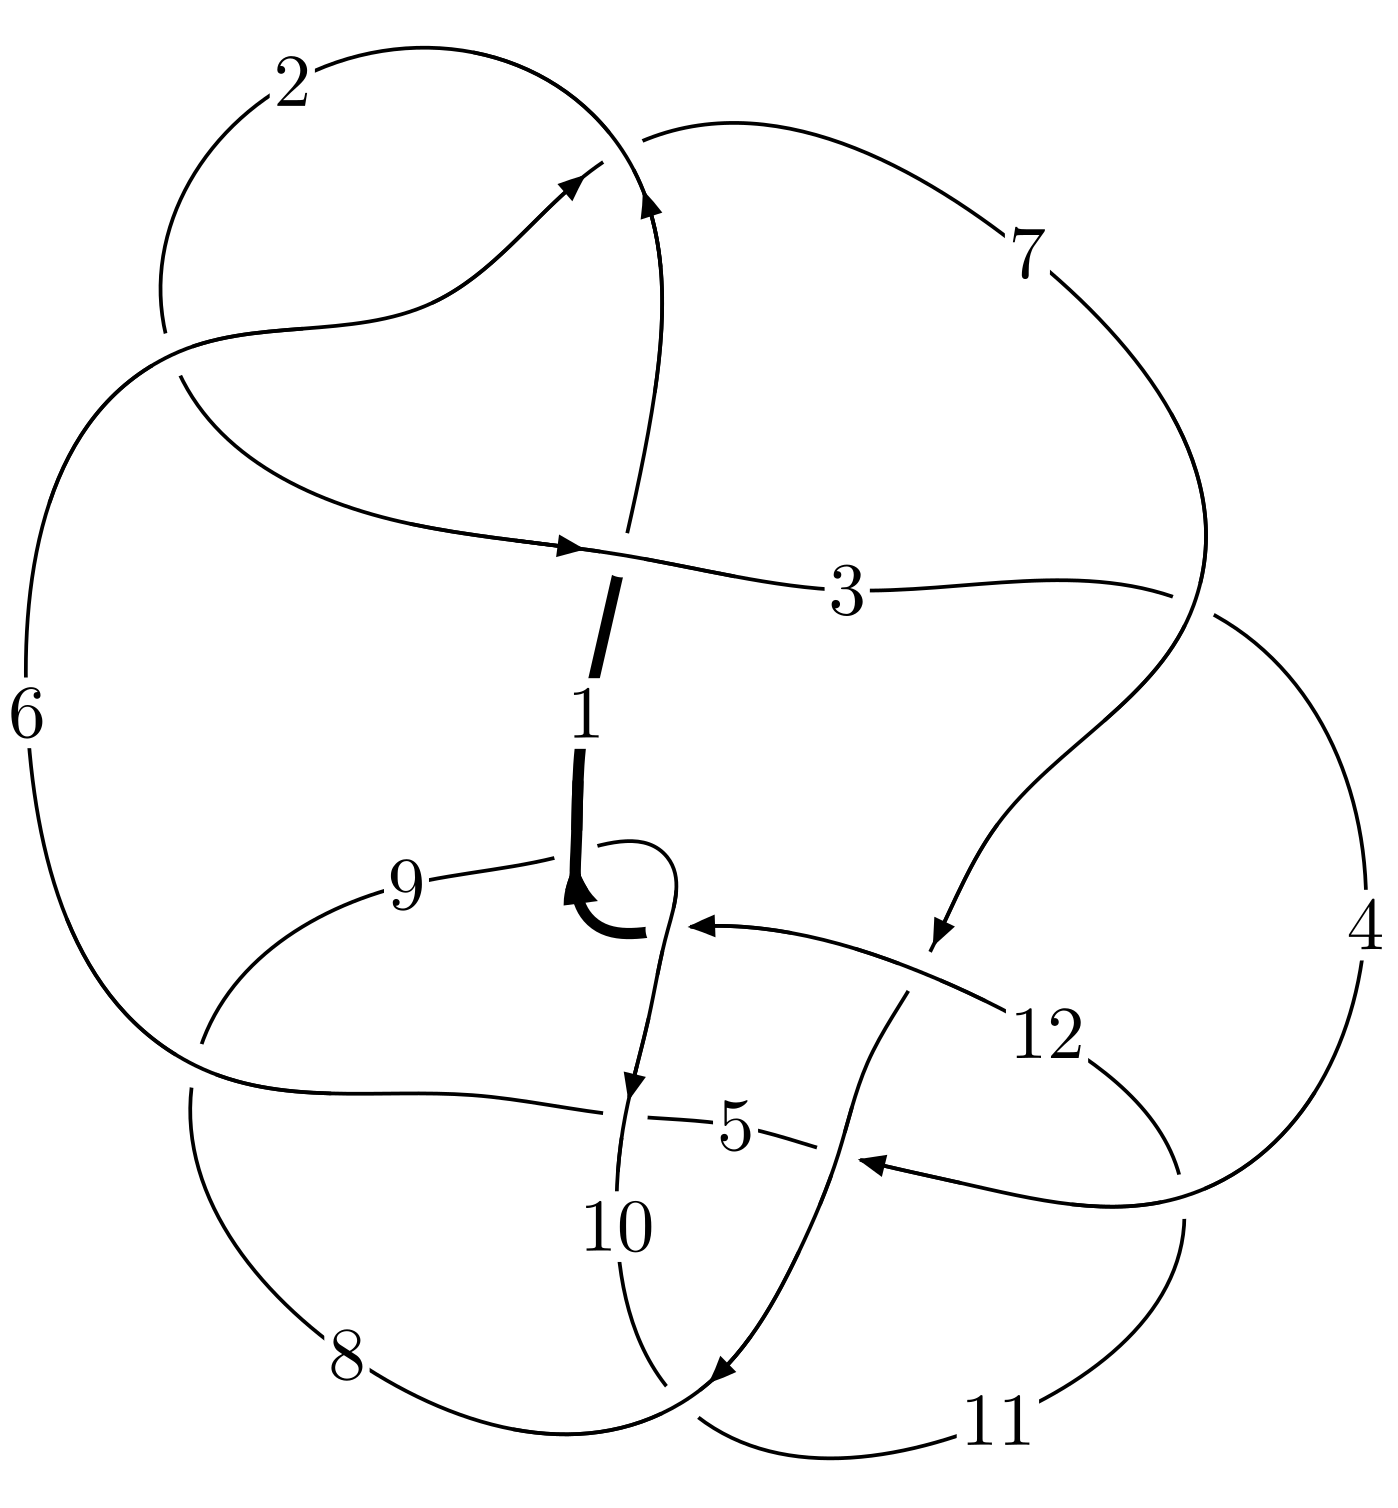
\includegraphics[width=112pt]{../../../GIT/diagram.site/Diagrams/png/2371_12n_0282.png}\\
\ \ \ A knot diagram\footnotemark}&
\allowdisplaybreaks
\textbf{Linearized knot diagam} \\
\cline{2-2}
 &
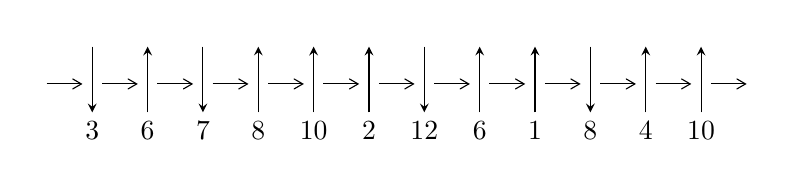
\begin{tikzpicture}[x=20pt, y=17pt]
	% nodes
	\node (C0) at (0, 0) {};
	\node (C1) at (1, 0) {};
	\node (C1U) at (1, +1) {};
	\node (C1D) at (1, -1) {3};

	\node (C2) at (2, 0) {};
	\node (C2U) at (2, +1) {};
	\node (C2D) at (2, -1) {6};

	\node (C3) at (3, 0) {};
	\node (C3U) at (3, +1) {};
	\node (C3D) at (3, -1) {7};

	\node (C4) at (4, 0) {};
	\node (C4U) at (4, +1) {};
	\node (C4D) at (4, -1) {8};

	\node (C5) at (5, 0) {};
	\node (C5U) at (5, +1) {};
	\node (C5D) at (5, -1) {10};

	\node (C6) at (6, 0) {};
	\node (C6U) at (6, +1) {};
	\node (C6D) at (6, -1) {2};

	\node (C7) at (7, 0) {};
	\node (C7U) at (7, +1) {};
	\node (C7D) at (7, -1) {12};

	\node (C8) at (8, 0) {};
	\node (C8U) at (8, +1) {};
	\node (C8D) at (8, -1) {6};

	\node (C9) at (9, 0) {};
	\node (C9U) at (9, +1) {};
	\node (C9D) at (9, -1) {1};

	\node (C10) at (10, 0) {};
	\node (C10U) at (10, +1) {};
	\node (C10D) at (10, -1) {8};

	\node (C11) at (11, 0) {};
	\node (C11U) at (11, +1) {};
	\node (C11D) at (11, -1) {4};

	\node (C12) at (12, 0) {};
	\node (C12U) at (12, +1) {};
	\node (C12D) at (12, -1) {10};
	\node (C13) at (13, 0) {};

	% arrows
	\draw[->,>={angle 60}]
	(C0) edge (C1) (C1) edge (C2) (C2) edge (C3) (C3) edge (C4) (C4) edge (C5) (C5) edge (C6) (C6) edge (C7) (C7) edge (C8) (C8) edge (C9) (C9) edge (C10) (C10) edge (C11) (C11) edge (C12) (C12) edge (C13) ;	\draw[->,>=stealth]
	(C1U) edge (C1D) (C2D) edge (C2U) (C3U) edge (C3D) (C4D) edge (C4U) (C5D) edge (C5U) (C6D) edge (C6U) (C7U) edge (C7D) (C8D) edge (C8U) (C9D) edge (C9U) (C10U) edge (C10D) (C11D) edge (C11U) (C12D) edge (C12U) ;
	\end{tikzpicture} \\
\hhline{~~} \\& 
\textbf{Solving Sequence} \\ \cline{2-2} 
 &
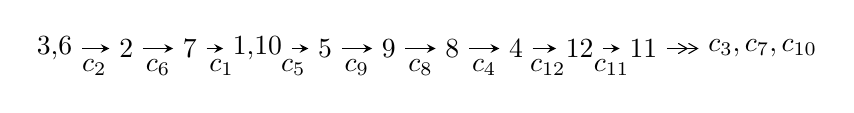
\begin{tikzpicture}[x=23pt, y=7pt]
	% node
	\node (A0) at (-1/8, 0) {3,6};
	\node (A1) at (1, 0) {2};
	\node (A2) at (2, 0) {7};
	\node (A3) at (49/16, 0) {1,10};
	\node (A4) at (33/8, 0) {5};
	\node (A5) at (41/8, 0) {9};
	\node (A6) at (49/8, 0) {8};
	\node (A7) at (57/8, 0) {4};
	\node (A8) at (65/8, 0) {12};
	\node (A9) at (73/8, 0) {11};
	\node (C1) at (1/2, -1) {$c_{2}$};
	\node (C2) at (3/2, -1) {$c_{6}$};
	\node (C3) at (5/2, -1) {$c_{1}$};
	\node (C4) at (29/8, -1) {$c_{5}$};
	\node (C5) at (37/8, -1) {$c_{9}$};
	\node (C6) at (45/8, -1) {$c_{8}$};
	\node (C7) at (53/8, -1) {$c_{4}$};
	\node (C8) at (61/8, -1) {$c_{12}$};
	\node (C9) at (69/8, -1) {$c_{11}$};
	\node (A10) at (11, 0) {$c_{3},c_{7},c_{10}$};

	% edge
	\draw[->,>=stealth]	
	(A0) edge (A1) (A1) edge (A2) (A2) edge (A3) (A3) edge (A4) (A4) edge (A5) (A5) edge (A6) (A6) edge (A7) (A7) edge (A8) (A8) edge (A9) ;
	\draw[->>,>={angle 60}]	
	(A9) edge (A10);
\end{tikzpicture} \\ 

\end{tabular} \\

\footnotetext{
The image of knot diagram is generated by the software ``\textbf{Draw programme}" developed by Andrew Bartholomew(\url{http://www.layer8.co.uk/maths/draw/index.htm\#Running-draw}), where we modified some parts for our purpose(\url{https://github.com/CATsTAILs/LinksPainter}).
}\phantom \\ \newline 
\centering \textbf{Ideals for irreducible components\footnotemark of $X_{\text{par}}$} 
 
\begin{align*}
I^u_{1}&=\langle 
u^{13}+3 u^{12}+9 u^{11}+16 u^{10}+26 u^9+32 u^8+33 u^7+28 u^6+17 u^5+9 u^4+u^3+u^2+b+1,\\
\phantom{I^u_{1}}&\phantom{= \langle  }u^{15}+5 u^{14}+\cdots+2 a+4,\;u^{16}+5 u^{15}+\cdots+4 u+2\rangle \\
I^u_{2}&=\langle 
u^{11}-2 u^{10}+5 u^9-7 u^8+9 u^7-11 u^6+10 u^5-10 u^4+6 u^3-4 u^2+b+3 u-1,\\
\phantom{I^u_{2}}&\phantom{= \langle  }u^{11}+2 u^9+2 u^8- u^7+4 u^6-6 u^5+5 u^4-8 u^3+3 u^2+2 a-2 u+3,\\
\phantom{I^u_{2}}&\phantom{= \langle  }u^{12}-2 u^{11}+6 u^{10}-8 u^9+13 u^8-14 u^7+16 u^6-15 u^5+12 u^4-9 u^3+6 u^2-3 u+2\rangle \\
I^u_{3}&=\langle 
- a u- u^2+b+u-1,\;u^2 a+a^2+5 u^2+a-2 u+7,\;u^3- u^2+2 u-1\rangle \\
\\
\end{align*}
\raggedright * 3 irreducible components of $\dim_{\mathbb{C}}=0$, with total 34 representations.\\
\footnotetext{All coefficients of polynomials are rational numbers. But the coefficients are sometimes approximated in decimal forms when there is not enough margin.}
\newpage
\renewcommand{\arraystretch}{1}
\centering \section*{I. $I^u_{1}= \langle u^{13}+3 u^{12}+\cdots+b+1,\;u^{15}+5 u^{14}+\cdots+2 a+4,\;u^{16}+5 u^{15}+\cdots+4 u+2 \rangle$}
\flushleft \textbf{(i) Arc colorings}\\
\begin{tabular}{m{7pt} m{180pt} m{7pt} m{180pt} }
\flushright $a_{3}=$&$\begin{pmatrix}1\\0\end{pmatrix}$ \\
\flushright $a_{6}=$&$\begin{pmatrix}0\\u\end{pmatrix}$ \\
\flushright $a_{2}=$&$\begin{pmatrix}1\\u^2\end{pmatrix}$ \\
\flushright $a_{7}=$&$\begin{pmatrix}u\\u^3+u\end{pmatrix}$ \\
\flushright $a_{1}=$&$\begin{pmatrix}u^2+1\\u^2\end{pmatrix}$ \\
\flushright $a_{10}=$&$\begin{pmatrix}-\frac{1}{2} u^{15}-\frac{5}{2} u^{14}+\cdots-\frac{5}{2} u-2\\- u^{13}-3 u^{12}+\cdots- u^2-1\end{pmatrix}$ \\
\flushright $a_{5}=$&$\begin{pmatrix}-\frac{1}{2} u^{15}-\frac{3}{2} u^{14}+\cdots- u^2-\frac{1}{2} u\\- u^{15}-4 u^{14}+\cdots- u-1\end{pmatrix}$ \\
\flushright $a_{9}=$&$\begin{pmatrix}\frac{1}{2} u^{15}+\frac{5}{2} u^{14}+\cdots+\frac{1}{2} u+1\\u^{14}+4 u^{13}+\cdots+2 u+1\end{pmatrix}$ \\
\flushright $a_{8}=$&$\begin{pmatrix}\frac{1}{2} u^{15}+\frac{5}{2} u^{14}+\cdots+\frac{1}{2} u+1\\- u^{14}- u^{13}+\cdots+u+1\end{pmatrix}$ \\
\flushright $a_{4}=$&$\begin{pmatrix}u^4+u^2+1\\u^6+2 u^4+u^2\end{pmatrix}$ \\
\flushright $a_{12}=$&$\begin{pmatrix}-\frac{1}{2} u^{15}-\frac{5}{2} u^{14}+\cdots-2 u^2-\frac{3}{2} u\\- u^{13}-3 u^{12}+\cdots- u-1\end{pmatrix}$ \\
\flushright $a_{11}=$&$\begin{pmatrix}-\frac{5}{2} u^{15}-\frac{25}{2} u^{14}+\cdots-\frac{15}{2} u-5\\u^{14}-4 u^{13}+\cdots-3 u-5\end{pmatrix}$\\&\end{tabular}
\flushleft \textbf{(ii) Obstruction class $= -1$}\\~\\
\flushleft \textbf{(iii) Cusp Shapes $= 3 u^{15}+14 u^{14}+49 u^{13}+118 u^{12}+232 u^{11}+373 u^{10}+501 u^9+574 u^8+544 u^7+435 u^6+280 u^5+141 u^4+62 u^3+25 u^2+20 u+14$}\\~\\
\newpage\renewcommand{\arraystretch}{1}
\flushleft \textbf{(iv) u-Polynomials at the component}\newline \\
\begin{tabular}{m{50pt}|m{274pt}}
Crossings & \hspace{64pt}u-Polynomials at each crossing \\
\hline $$\begin{aligned}c_{1}\end{aligned}$$&$\begin{aligned}
&u^{16}+11 u^{15}+\cdots+12 u+4
\end{aligned}$\\
\hline $$\begin{aligned}c_{2},c_{6}\end{aligned}$$&$\begin{aligned}
&u^{16}-5 u^{15}+\cdots-4 u+2
\end{aligned}$\\
\hline $$\begin{aligned}c_{3}\end{aligned}$$&$\begin{aligned}
&u^{16}+5 u^{15}+\cdots-4 u+10
\end{aligned}$\\
\hline $$\begin{aligned}c_{4},c_{5},c_{11}\end{aligned}$$&$\begin{aligned}
&u^{16}+13 u^{14}+\cdots- u+1
\end{aligned}$\\
\hline $$\begin{aligned}c_{7}\end{aligned}$$&$\begin{aligned}
&u^{16}+9 u^{15}+\cdots+24 u+8
\end{aligned}$\\
\hline $$\begin{aligned}c_{8}\end{aligned}$$&$\begin{aligned}
&u^{16}+u^{15}+\cdots-487 u+889
\end{aligned}$\\
\hline $$\begin{aligned}c_{9},c_{12}\end{aligned}$$&$\begin{aligned}
&u^{16}-2 u^{15}+\cdots-17 u+1
\end{aligned}$\\
\hline $$\begin{aligned}c_{10}\end{aligned}$$&$\begin{aligned}
&u^{16}-17 u^{15}+\cdots-52 u+10
\end{aligned}$\\
\hline
\end{tabular}\\~\\
\newpage\renewcommand{\arraystretch}{1}
\flushleft \textbf{(v) Riley Polynomials at the component}\newline \\
\begin{tabular}{m{50pt}|m{274pt}}
Crossings & \hspace{64pt}Riley Polynomials at each crossing \\
\hline $$\begin{aligned}c_{1}\end{aligned}$$&$\begin{aligned}
&y^{16}-9 y^{15}+\cdots+632 y+16
\end{aligned}$\\
\hline $$\begin{aligned}c_{2},c_{6}\end{aligned}$$&$\begin{aligned}
&y^{16}+11 y^{15}+\cdots+12 y+4
\end{aligned}$\\
\hline $$\begin{aligned}c_{3}\end{aligned}$$&$\begin{aligned}
&y^{16}-41 y^{15}+\cdots+764 y+100
\end{aligned}$\\
\hline $$\begin{aligned}c_{4},c_{5},c_{11}\end{aligned}$$&$\begin{aligned}
&y^{16}+26 y^{15}+\cdots+7 y+1
\end{aligned}$\\
\hline $$\begin{aligned}c_{7}\end{aligned}$$&$\begin{aligned}
&y^{16}+3 y^{15}+\cdots+288 y+64
\end{aligned}$\\
\hline $$\begin{aligned}c_{8}\end{aligned}$$&$\begin{aligned}
&y^{16}+109 y^{15}+\cdots-11168313 y+790321
\end{aligned}$\\
\hline $$\begin{aligned}c_{9},c_{12}\end{aligned}$$&$\begin{aligned}
&y^{16}+34 y^{15}+\cdots-47 y+1
\end{aligned}$\\
\hline $$\begin{aligned}c_{10}\end{aligned}$$&$\begin{aligned}
&y^{16}-49 y^{15}+\cdots+36 y+100
\end{aligned}$\\
\hline
\end{tabular}\\~\\
\newpage\flushleft \textbf{(vi) Complex Volumes and Cusp Shapes}
$$\begin{array}{c|c|c}  
\text{Solutions to }I^u_{1}& \I (\text{vol} + \sqrt{-1}CS) & \text{Cusp shape}\\
 \hline 
\begin{aligned}
u &= -0.478305 + 1.028310 I \\
a &= \phantom{-}0.050929 + 0.582193 I \\
b &= \phantom{-}0.623036 + 0.226095 I\end{aligned}
 & -0.64871 - 3.08703 I & \phantom{-}2.33099 + 0.59290 I \\ \hline\begin{aligned}
u &= -0.478305 - 1.028310 I \\
a &= \phantom{-}0.050929 - 0.582193 I \\
b &= \phantom{-}0.623036 - 0.226095 I\end{aligned}
 & -0.64871 + 3.08703 I & \phantom{-}2.33099 - 0.59290 I \\ \hline\begin{aligned}
u &= -1.136630 + 0.036859 I \\
a &= \phantom{-}0.25201 - 1.80758 I \\
b &= \phantom{-}0.21982 - 2.06384 I\end{aligned}
 & -19.1158 - 4.5602 I & \phantom{-}1.43322 + 1.94202 I \\ \hline\begin{aligned}
u &= -1.136630 - 0.036859 I \\
a &= \phantom{-}0.25201 + 1.80758 I \\
b &= \phantom{-}0.21982 + 2.06384 I\end{aligned}
 & -19.1158 + 4.5602 I & \phantom{-}1.43322 - 1.94202 I \\ \hline\begin{aligned}
u &= \phantom{-}0.065300 + 1.174500 I \\
a &= \phantom{-}0.511213 + 0.476614 I \\
b &= \phantom{-}0.526402 - 0.631543 I\end{aligned}
 & -3.55568 - 0.83919 I & -1.52217 + 2.21836 I \\ \hline\begin{aligned}
u &= \phantom{-}0.065300 - 1.174500 I \\
a &= \phantom{-}0.511213 - 0.476614 I \\
b &= \phantom{-}0.526402 + 0.631543 I\end{aligned}
 & -3.55568 + 0.83919 I & -1.52217 - 2.21836 I \\ \hline\begin{aligned}
u &= \phantom{-}0.284247 + 1.175830 I \\
a &= -0.458912 - 0.456538 I \\
b &= -0.406366 + 0.669372 I\end{aligned}
 & -1.92269 + 4.32175 I & -1.05745 - 3.72733 I \\ \hline\begin{aligned}
u &= \phantom{-}0.284247 - 1.175830 I \\
a &= -0.458912 + 0.456538 I \\
b &= -0.406366 - 0.669372 I\end{aligned}
 & -1.92269 - 4.32175 I & -1.05745 + 3.72733 I \\ \hline\begin{aligned}
u &= -0.462160 + 0.504593 I \\
a &= -0.810441 - 0.051513 I \\
b &= -0.400547 + 0.385135 I\end{aligned}
 & \phantom{-}0.900558 - 0.884001 I & \phantom{-}7.79246 + 5.53646 I \\ \hline\begin{aligned}
u &= -0.462160 - 0.504593 I \\
a &= -0.810441 + 0.051513 I \\
b &= -0.400547 - 0.385135 I\end{aligned}
 & \phantom{-}0.900558 + 0.884001 I & \phantom{-}7.79246 - 5.53646 I\\
 \hline 
 \end{array}$$\newpage$$\begin{array}{c|c|c}  
\text{Solutions to }I^u_{1}& \I (\text{vol} + \sqrt{-1}CS) & \text{Cusp shape}\\
 \hline 
\begin{aligned}
u &= -0.59084 + 1.38518 I \\
a &= \phantom{-}1.216170 - 0.591623 I \\
b &= -0.10095 - 2.03417 I\end{aligned}
 & \phantom{-}16.1808 - 1.5728 I & -0.910122 + 0.801977 I \\ \hline\begin{aligned}
u &= -0.59084 - 1.38518 I \\
a &= \phantom{-}1.216170 + 0.591623 I \\
b &= -0.10095 + 2.03417 I\end{aligned}
 & \phantom{-}16.1808 + 1.5728 I & -0.910122 - 0.801977 I \\ \hline\begin{aligned}
u &= \phantom{-}0.364622 + 0.333050 I \\
a &= -0.375430 - 0.860631 I \\
b &= -0.149743 + 0.438842 I\end{aligned}
 & \phantom{-}0.56988 - 1.44730 I & \phantom{-}4.97392 + 6.26939 I \\ \hline\begin{aligned}
u &= \phantom{-}0.364622 - 0.333050 I \\
a &= -0.375430 + 0.860631 I \\
b &= -0.149743 - 0.438842 I\end{aligned}
 & \phantom{-}0.56988 + 1.44730 I & \phantom{-}4.97392 - 6.26939 I \\ \hline\begin{aligned}
u &= -0.54623 + 1.41233 I \\
a &= -1.38554 + 0.31520 I \\
b &= -0.31165 + 2.12901 I\end{aligned}
 & \phantom{-}15.8163 - 10.5372 I & -1.04085 + 4.44511 I \\ \hline\begin{aligned}
u &= -0.54623 - 1.41233 I \\
a &= -1.38554 - 0.31520 I \\
b &= -0.31165 - 2.12901 I\end{aligned}
 & \phantom{-}15.8163 + 10.5372 I & -1.04085 - 4.44511 I\\
 \hline 
 \end{array}$$\newpage\newpage\renewcommand{\arraystretch}{1}
\centering \section*{II. $I^u_{2}= \langle u^{11}-2 u^{10}+\cdots+b-1,\;u^{11}+2 u^9+\cdots+2 a+3,\;u^{12}-2 u^{11}+\cdots-3 u+2 \rangle$}
\flushleft \textbf{(i) Arc colorings}\\
\begin{tabular}{m{7pt} m{180pt} m{7pt} m{180pt} }
\flushright $a_{3}=$&$\begin{pmatrix}1\\0\end{pmatrix}$ \\
\flushright $a_{6}=$&$\begin{pmatrix}0\\u\end{pmatrix}$ \\
\flushright $a_{2}=$&$\begin{pmatrix}1\\u^2\end{pmatrix}$ \\
\flushright $a_{7}=$&$\begin{pmatrix}u\\u^3+u\end{pmatrix}$ \\
\flushright $a_{1}=$&$\begin{pmatrix}u^2+1\\u^2\end{pmatrix}$ \\
\flushright $a_{10}=$&$\begin{pmatrix}-\frac{1}{2} u^{11}- u^9+\cdots+u-\frac{3}{2}\\- u^{11}+2 u^{10}+\cdots-3 u+1\end{pmatrix}$ \\
\flushright $a_{5}=$&$\begin{pmatrix}-\frac{3}{2} u^{11}+3 u^{10}+\cdots-5 u+\frac{5}{2}\\u^{10}-2 u^9+5 u^8-6 u^7+8 u^6-8 u^5+8 u^4-7 u^3+4 u^2- u+3\end{pmatrix}$ \\
\flushright $a_{9}=$&$\begin{pmatrix}-\frac{1}{2} u^{11}- u^9+\cdots+\frac{1}{2} u^2-\frac{1}{2}\\- u^{11}+2 u^{10}+\cdots-3 u+1\end{pmatrix}$ \\
\flushright $a_{8}=$&$\begin{pmatrix}-\frac{1}{2} u^{11}- u^9+\cdots+\frac{1}{2} u^2-\frac{1}{2}\\- u^{11}+3 u^{10}+\cdots-5 u+3\end{pmatrix}$ \\
\flushright $a_{4}=$&$\begin{pmatrix}u^4+u^2+1\\u^6+2 u^4+u^2\end{pmatrix}$ \\
\flushright $a_{12}=$&$\begin{pmatrix}\frac{1}{2} u^{11}+u^9+\cdots+\frac{1}{2} u^2+\frac{3}{2}\\u^{11}-2 u^{10}+5 u^9-6 u^8+8 u^7-8 u^6+8 u^5-7 u^4+4 u^3-2 u^2+2 u-1\end{pmatrix}$ \\
\flushright $a_{11}=$&$\begin{pmatrix}\frac{1}{2} u^{11}+u^9+\cdots-\frac{1}{2} u^2+\frac{1}{2}\\u^{11}-3 u^{10}+\cdots+3 u-3\end{pmatrix}$\\&\end{tabular}
\flushleft \textbf{(ii) Obstruction class $= 1$}\\~\\
\flushleft \textbf{(iii) Cusp Shapes $= u^{11}-5 u^{10}+10 u^9-21 u^8+24 u^7-31 u^6+28 u^5-25 u^4+22 u^3-12 u^2+8 u-4$}\\~\\
\newpage\renewcommand{\arraystretch}{1}
\flushleft \textbf{(iv) u-Polynomials at the component}\newline \\
\begin{tabular}{m{50pt}|m{274pt}}
Crossings & \hspace{64pt}u-Polynomials at each crossing \\
\hline $$\begin{aligned}c_{1}\end{aligned}$$&$\begin{aligned}
&u^{12}-8 u^{11}+\cdots-15 u+4
\end{aligned}$\\
\hline $$\begin{aligned}c_{2}\end{aligned}$$&$\begin{aligned}
&u^{12}-2 u^{11}+\cdots-3 u+2
\end{aligned}$\\
\hline $$\begin{aligned}c_{3}\end{aligned}$$&$\begin{aligned}
&u^{12}+2 u^{11}-2 u^9+6 u^8+10 u^7+5 u^6+2 u^5+11 u^4+u^3+4 u^2+5 u+2
\end{aligned}$\\
\hline $$\begin{aligned}c_{4},c_{11}\end{aligned}$$&$\begin{aligned}
&u^{12}+8 u^{10}+\cdots-2 u+1
\end{aligned}$\\
\hline $$\begin{aligned}c_{5}\end{aligned}$$&$\begin{aligned}
&u^{12}+8 u^{10}+\cdots+2 u+1
\end{aligned}$\\
\hline $$\begin{aligned}c_{6}\end{aligned}$$&$\begin{aligned}
&u^{12}+2 u^{11}+\cdots+3 u+2
\end{aligned}$\\
\hline $$\begin{aligned}c_{7}\end{aligned}$$&$\begin{aligned}
&u^{12}+2 u^{11}+\cdots+2 u+1
\end{aligned}$\\
\hline $$\begin{aligned}c_{8}\end{aligned}$$&$\begin{aligned}
&u^{12}+5 u^{11}+\cdots-7 u^2+1
\end{aligned}$\\
\hline $$\begin{aligned}c_{9}\end{aligned}$$&$\begin{aligned}
&u^{12}-2 u^{11}+\cdots-2 u+1
\end{aligned}$\\
\hline $$\begin{aligned}c_{10}\end{aligned}$$&$\begin{aligned}
&u^{12}+14 u^{11}+\cdots+495 u+80
\end{aligned}$\\
\hline $$\begin{aligned}c_{12}\end{aligned}$$&$\begin{aligned}
&u^{12}+2 u^{11}+\cdots+2 u+1
\end{aligned}$\\
\hline
\end{tabular}\\~\\
\newpage\renewcommand{\arraystretch}{1}
\flushleft \textbf{(v) Riley Polynomials at the component}\newline \\
\begin{tabular}{m{50pt}|m{274pt}}
Crossings & \hspace{64pt}Riley Polynomials at each crossing \\
\hline $$\begin{aligned}c_{1}\end{aligned}$$&$\begin{aligned}
&y^{12}-4 y^{11}+\cdots+15 y+16
\end{aligned}$\\
\hline $$\begin{aligned}c_{2},c_{6}\end{aligned}$$&$\begin{aligned}
&y^{12}+8 y^{11}+\cdots+15 y+4
\end{aligned}$\\
\hline $$\begin{aligned}c_{3}\end{aligned}$$&$\begin{aligned}
&y^{12}-4 y^{11}+\cdots-9 y+4
\end{aligned}$\\
\hline $$\begin{aligned}c_{4},c_{5},c_{11}\end{aligned}$$&$\begin{aligned}
&y^{12}+16 y^{11}+\cdots+2 y+1
\end{aligned}$\\
\hline $$\begin{aligned}c_{7}\end{aligned}$$&$\begin{aligned}
&y^{12}+4 y^{11}+\cdots+8 y+1
\end{aligned}$\\
\hline $$\begin{aligned}c_{8}\end{aligned}$$&$\begin{aligned}
&y^{12}-13 y^{11}+\cdots-14 y+1
\end{aligned}$\\
\hline $$\begin{aligned}c_{9},c_{12}\end{aligned}$$&$\begin{aligned}
&y^{12}+8 y^{11}+\cdots+4 y+1
\end{aligned}$\\
\hline $$\begin{aligned}c_{10}\end{aligned}$$&$\begin{aligned}
&y^{12}-8 y^{11}+\cdots+3615 y+6400
\end{aligned}$\\
\hline
\end{tabular}\\~\\
\newpage\flushleft \textbf{(vi) Complex Volumes and Cusp Shapes}
$$\begin{array}{c|c|c}  
\text{Solutions to }I^u_{2}& \I (\text{vol} + \sqrt{-1}CS) & \text{Cusp shape}\\
 \hline 
\begin{aligned}
u &= \phantom{-}0.249672 + 0.959195 I \\
a &= -1.68135 - 0.45806 I \\
b &= \phantom{-}0.01959 - 1.72711 I\end{aligned}
 & -7.94302 + 1.00045 I & -2.72933 - 0.10711 I \\ \hline\begin{aligned}
u &= \phantom{-}0.249672 - 0.959195 I \\
a &= -1.68135 + 0.45806 I \\
b &= \phantom{-}0.01959 + 1.72711 I\end{aligned}
 & -7.94302 - 1.00045 I & -2.72933 + 0.10711 I \\ \hline\begin{aligned}
u &= -0.429646 + 0.953539 I \\
a &= -0.073134 - 0.459239 I \\
b &= \phantom{-}0.469324 + 0.127574 I\end{aligned}
 & -0.45876 - 4.18304 I & \phantom{-}4.58234 + 6.10453 I \\ \hline\begin{aligned}
u &= -0.429646 - 0.953539 I \\
a &= -0.073134 + 0.459239 I \\
b &= \phantom{-}0.469324 - 0.127574 I\end{aligned}
 & -0.45876 + 4.18304 I & \phantom{-}4.58234 - 6.10453 I \\ \hline\begin{aligned}
u &= \phantom{-}0.839161 + 0.302874 I \\
a &= \phantom{-}0.461054 + 1.306310 I \\
b &= -0.008748 + 1.235850 I\end{aligned}
 & -2.36446 - 1.00466 I & \phantom{-}2.85304 + 0.63873 I \\ \hline\begin{aligned}
u &= \phantom{-}0.839161 - 0.302874 I \\
a &= \phantom{-}0.461054 - 1.306310 I \\
b &= -0.008748 - 1.235850 I\end{aligned}
 & -2.36446 + 1.00466 I & \phantom{-}2.85304 - 0.63873 I \\ \hline\begin{aligned}
u &= -0.484489 + 0.716111 I \\
a &= \phantom{-}0.556723 - 0.092910 I \\
b &= -0.203192 + 0.443689 I\end{aligned}
 & \phantom{-}0.268555 + 0.420031 I & \phantom{-}1.039574 + 0.824157 I \\ \hline\begin{aligned}
u &= -0.484489 - 0.716111 I \\
a &= \phantom{-}0.556723 + 0.092910 I \\
b &= -0.203192 - 0.443689 I\end{aligned}
 & \phantom{-}0.268555 - 0.420031 I & \phantom{-}1.039574 - 0.824157 I \\ \hline\begin{aligned}
u &= \phantom{-}0.581682 + 1.140840 I \\
a &= \phantom{-}1.010720 + 0.383459 I \\
b &= \phantom{-}0.150456 + 1.376120 I\end{aligned}
 & -4.83530 + 6.22925 I & \phantom{-}0.60260 - 5.56850 I \\ \hline\begin{aligned}
u &= \phantom{-}0.581682 - 1.140840 I \\
a &= \phantom{-}1.010720 - 0.383459 I \\
b &= \phantom{-}0.150456 - 1.376120 I\end{aligned}
 & -4.83530 - 6.22925 I & \phantom{-}0.60260 + 5.56850 I\\
 \hline 
 \end{array}$$\newpage$$\begin{array}{c|c|c}  
\text{Solutions to }I^u_{2}& \I (\text{vol} + \sqrt{-1}CS) & \text{Cusp shape}\\
 \hline 
\begin{aligned}
u &= \phantom{-}0.243620 + 1.359490 I \\
a &= -1.024010 + 0.130899 I \\
b &= -0.42743 - 1.36024 I\end{aligned}
 & -7.69609 + 2.59197 I & -0.34822 - 1.94419 I \\ \hline\begin{aligned}
u &= \phantom{-}0.243620 - 1.359490 I \\
a &= -1.024010 - 0.130899 I \\
b &= -0.42743 + 1.36024 I\end{aligned}
 & -7.69609 - 2.59197 I & -0.34822 + 1.94419 I\\
 \hline 
 \end{array}$$\newpage\newpage\renewcommand{\arraystretch}{1}
\centering \section*{III. $I^u_{3}= \langle - a u- u^2+b+u-1,\;u^2 a+a^2+5 u^2+a-2 u+7,\;u^3- u^2+2 u-1 \rangle$}
\flushleft \textbf{(i) Arc colorings}\\
\begin{tabular}{m{7pt} m{180pt} m{7pt} m{180pt} }
\flushright $a_{3}=$&$\begin{pmatrix}1\\0\end{pmatrix}$ \\
\flushright $a_{6}=$&$\begin{pmatrix}0\\u\end{pmatrix}$ \\
\flushright $a_{2}=$&$\begin{pmatrix}1\\u^2\end{pmatrix}$ \\
\flushright $a_{7}=$&$\begin{pmatrix}u\\u^2- u+1\end{pmatrix}$ \\
\flushright $a_{1}=$&$\begin{pmatrix}u^2+1\\u^2\end{pmatrix}$ \\
\flushright $a_{10}=$&$\begin{pmatrix}a\\a u+u^2- u+1\end{pmatrix}$ \\
\flushright $a_{5}=$&$\begin{pmatrix}u^2 a- a u+3 u^2+a-3 u+5\\3\end{pmatrix}$ \\
\flushright $a_{9}=$&$\begin{pmatrix}- a u- u^2+a-1\\- a u+a- u+1\end{pmatrix}$ \\
\flushright $a_{8}=$&$\begin{pmatrix}- a u- u^2+a-1\\a u\end{pmatrix}$ \\
\flushright $a_{4}=$&$\begin{pmatrix}- u+2\\u\end{pmatrix}$ \\
\flushright $a_{12}=$&$\begin{pmatrix}- a u- u^2+a- u-1\\a u- u^2+u-1\end{pmatrix}$ \\
\flushright $a_{11}=$&$\begin{pmatrix}u^2 a-3 a u- u^2+a- u-1\\- u^2 a+a u- u^2+u-1\end{pmatrix}$\\&\end{tabular}
\flushleft \textbf{(ii) Obstruction class $= -1$}\\~\\
\flushleft \textbf{(iii) Cusp Shapes $= 4 u^2-4 u+2$}\\~\\
\newpage\renewcommand{\arraystretch}{1}
\flushleft \textbf{(iv) u-Polynomials at the component}\newline \\
\begin{tabular}{m{50pt}|m{274pt}}
Crossings & \hspace{64pt}u-Polynomials at each crossing \\
\hline $$\begin{aligned}c_{1}\end{aligned}$$&$\begin{aligned}
&(u^3+3 u^2+2 u-1)^2
\end{aligned}$\\
\hline $$\begin{aligned}c_{2},c_{6}\end{aligned}$$&$\begin{aligned}
&(u^3+u^2+2 u+1)^2
\end{aligned}$\\
\hline $$\begin{aligned}c_{3}\end{aligned}$$&$\begin{aligned}
&(u^3- u^2+1)^2
\end{aligned}$\\
\hline $$\begin{aligned}c_{4},c_{5},c_{11}\end{aligned}$$&$\begin{aligned}
&u^6- u^5+8 u^4-2 u^3+24 u^2+23
\end{aligned}$\\
\hline $$\begin{aligned}c_{7}\end{aligned}$$&$\begin{aligned}
&(u-1)^6
\end{aligned}$\\
\hline $$\begin{aligned}c_{8}\end{aligned}$$&$\begin{aligned}
&u^6-5 u^5-6 u^4+30 u^3+78 u^2+70 u+23
\end{aligned}$\\
\hline $$\begin{aligned}c_{9},c_{12}\end{aligned}$$&$\begin{aligned}
&u^6+5 u^5+18 u^4+28 u^3+42 u^2+30 u+25
\end{aligned}$\\
\hline $$\begin{aligned}c_{10}\end{aligned}$$&$\begin{aligned}
&(u^3+5 u^2+10 u+7)^2
\end{aligned}$\\
\hline
\end{tabular}\\~\\
\newpage\renewcommand{\arraystretch}{1}
\flushleft \textbf{(v) Riley Polynomials at the component}\newline \\
\begin{tabular}{m{50pt}|m{274pt}}
Crossings & \hspace{64pt}Riley Polynomials at each crossing \\
\hline $$\begin{aligned}c_{1}\end{aligned}$$&$\begin{aligned}
&(y^3-5 y^2+10 y-1)^2
\end{aligned}$\\
\hline $$\begin{aligned}c_{2},c_{6}\end{aligned}$$&$\begin{aligned}
&(y^3+3 y^2+2 y-1)^2
\end{aligned}$\\
\hline $$\begin{aligned}c_{3}\end{aligned}$$&$\begin{aligned}
&(y^3- y^2+2 y-1)^2
\end{aligned}$\\
\hline $$\begin{aligned}c_{4},c_{5},c_{11}\end{aligned}$$&$\begin{aligned}
&y^6+15 y^5+108 y^4+426 y^3+944 y^2+1104 y+529
\end{aligned}$\\
\hline $$\begin{aligned}c_{7}\end{aligned}$$&$\begin{aligned}
&(y-1)^6
\end{aligned}$\\
\hline $$\begin{aligned}c_{8}\end{aligned}$$&$\begin{aligned}
&y^6-37 y^5+492 y^4-1090 y^3+1608 y^2-1312 y+529
\end{aligned}$\\
\hline $$\begin{aligned}c_{9},c_{12}\end{aligned}$$&$\begin{aligned}
&y^6+11 y^5+128 y^4+478 y^3+984 y^2+1200 y+625
\end{aligned}$\\
\hline $$\begin{aligned}c_{10}\end{aligned}$$&$\begin{aligned}
&(y^3-5 y^2+30 y-49)^2
\end{aligned}$\\
\hline
\end{tabular}\\~\\
\newpage\flushleft \textbf{(vi) Complex Volumes and Cusp Shapes}
$$\begin{array}{c|c|c}  
\text{Solutions to }I^u_{3}& \I (\text{vol} + \sqrt{-1}CS) & \text{Cusp shape}\\
 \hline 
\begin{aligned}
u &= \phantom{-}0.215080 + 1.307140 I \\
a &= -1.007880 - 0.138006 I \\
b &= -0.91382 - 2.09199 I\end{aligned}
 & -9.60386 + 2.82812 I & -5.50976 - 2.97945 I \\ \hline\begin{aligned}
u &= \phantom{-}0.215080 + 1.307140 I \\
a &= \phantom{-}1.67024 - 0.42427 I \\
b &= \phantom{-}0.036382 + 1.347130 I\end{aligned}
 & -9.60386 + 2.82812 I & -5.50976 - 2.97945 I \\ \hline\begin{aligned}
u &= \phantom{-}0.215080 - 1.307140 I \\
a &= -1.007880 + 0.138006 I \\
b &= -0.91382 + 2.09199 I\end{aligned}
 & -9.60386 - 2.82812 I & -5.50976 + 2.97945 I \\ \hline\begin{aligned}
u &= \phantom{-}0.215080 - 1.307140 I \\
a &= \phantom{-}1.67024 + 0.42427 I \\
b &= \phantom{-}0.036382 - 1.347130 I\end{aligned}
 & -9.60386 - 2.82812 I & -5.50976 + 2.97945 I \\ \hline\begin{aligned}
u &= \phantom{-}0.569840\phantom{ +0.000000I} \\
a &= -0.66236 + 2.65428 I \\
b &= \phantom{-}0.37744 + 1.51251 I\end{aligned}
 & -5.46628\phantom{ +0.000000I} & \phantom{-}1.01950\phantom{ +0.000000I} \\ \hline\begin{aligned}
u &= \phantom{-}0.569840\phantom{ +0.000000I} \\
a &= -0.66236 - 2.65428 I \\
b &= \phantom{-}0.37744 - 1.51251 I\end{aligned}
 & -5.46628\phantom{ +0.000000I} & \phantom{-}1.01950\phantom{ +0.000000I}\\
 \hline 
 \end{array}$$\newpage
\newpage\renewcommand{\arraystretch}{1}
\centering \section*{ IV. u-Polynomials}
\begin{tabular}{m{50pt}|m{274pt}}
Crossings & \hspace{64pt}u-Polynomials at each crossing \\
\hline $$\begin{aligned}c_{1}\end{aligned}$$&$\begin{aligned}
&((u^3+3 u^2+2 u-1)^2)(u^{12}-8 u^{11}+\cdots-15 u+4)\\
&\cdot(u^{16}+11 u^{15}+\cdots+12 u+4)
\end{aligned}$\\
\hline $$\begin{aligned}c_{2}\end{aligned}$$&$\begin{aligned}
&((u^3+u^2+2 u+1)^2)(u^{12}-2 u^{11}+\cdots-3 u+2)\\
&\cdot(u^{16}-5 u^{15}+\cdots-4 u+2)
\end{aligned}$\\
\hline $$\begin{aligned}c_{3}\end{aligned}$$&$\begin{aligned}
&(u^3- u^2+1)^2\\
&\cdot(u^{12}+2 u^{11}-2 u^9+6 u^8+10 u^7+5 u^6+2 u^5+11 u^4+u^3+4 u^2+5 u+2)\\
&\cdot(u^{16}+5 u^{15}+\cdots-4 u+10)
\end{aligned}$\\
\hline $$\begin{aligned}c_{4},c_{11}\end{aligned}$$&$\begin{aligned}
&(u^6- u^5+8 u^4-2 u^3+24 u^2+23)(u^{12}+8 u^{10}+\cdots-2 u+1)\\
&\cdot(u^{16}+13 u^{14}+\cdots- u+1)
\end{aligned}$\\
\hline $$\begin{aligned}c_{5}\end{aligned}$$&$\begin{aligned}
&(u^6- u^5+8 u^4-2 u^3+24 u^2+23)(u^{12}+8 u^{10}+\cdots+2 u+1)\\
&\cdot(u^{16}+13 u^{14}+\cdots- u+1)
\end{aligned}$\\
\hline $$\begin{aligned}c_{6}\end{aligned}$$&$\begin{aligned}
&((u^3+u^2+2 u+1)^2)(u^{12}+2 u^{11}+\cdots+3 u+2)\\
&\cdot(u^{16}-5 u^{15}+\cdots-4 u+2)
\end{aligned}$\\
\hline $$\begin{aligned}c_{7}\end{aligned}$$&$\begin{aligned}
&((u-1)^6)(u^{12}+2 u^{11}+\cdots+2 u+1)(u^{16}+9 u^{15}+\cdots+24 u+8)
\end{aligned}$\\
\hline $$\begin{aligned}c_{8}\end{aligned}$$&$\begin{aligned}
&(u^6-5 u^5+\cdots+70 u+23)(u^{12}+5 u^{11}+\cdots-7 u^2+1)\\
&\cdot(u^{16}+u^{15}+\cdots-487 u+889)
\end{aligned}$\\
\hline $$\begin{aligned}c_{9}\end{aligned}$$&$\begin{aligned}
&(u^6+5 u^5+\cdots+30 u+25)(u^{12}-2 u^{11}+\cdots-2 u+1)\\
&\cdot(u^{16}-2 u^{15}+\cdots-17 u+1)
\end{aligned}$\\
\hline $$\begin{aligned}c_{10}\end{aligned}$$&$\begin{aligned}
&((u^3+5 u^2+10 u+7)^2)(u^{12}+14 u^{11}+\cdots+495 u+80)\\
&\cdot(u^{16}-17 u^{15}+\cdots-52 u+10)
\end{aligned}$\\
\hline $$\begin{aligned}c_{12}\end{aligned}$$&$\begin{aligned}
&(u^6+5 u^5+\cdots+30 u+25)(u^{12}+2 u^{11}+\cdots+2 u+1)\\
&\cdot(u^{16}-2 u^{15}+\cdots-17 u+1)
\end{aligned}$\\
\hline
\end{tabular}\newpage\renewcommand{\arraystretch}{1}
\centering \section*{ V. Riley Polynomials}
\begin{tabular}{m{50pt}|m{274pt}}
Crossings & \hspace{64pt}Riley Polynomials at each crossing \\
\hline $$\begin{aligned}c_{1}\end{aligned}$$&$\begin{aligned}
&((y^3-5 y^2+10 y-1)^2)(y^{12}-4 y^{11}+\cdots+15 y+16)\\
&\cdot(y^{16}-9 y^{15}+\cdots+632 y+16)
\end{aligned}$\\
\hline $$\begin{aligned}c_{2},c_{6}\end{aligned}$$&$\begin{aligned}
&((y^3+3 y^2+2 y-1)^2)(y^{12}+8 y^{11}+\cdots+15 y+4)\\
&\cdot(y^{16}+11 y^{15}+\cdots+12 y+4)
\end{aligned}$\\
\hline $$\begin{aligned}c_{3}\end{aligned}$$&$\begin{aligned}
&((y^3- y^2+2 y-1)^2)(y^{12}-4 y^{11}+\cdots-9 y+4)\\
&\cdot(y^{16}-41 y^{15}+\cdots+764 y+100)
\end{aligned}$\\
\hline $$\begin{aligned}c_{4},c_{5},c_{11}\end{aligned}$$&$\begin{aligned}
&(y^6+15 y^5+108 y^4+426 y^3+944 y^2+1104 y+529)\\
&\cdot(y^{12}+16 y^{11}+\cdots+2 y+1)(y^{16}+26 y^{15}+\cdots+7 y+1)
\end{aligned}$\\
\hline $$\begin{aligned}c_{7}\end{aligned}$$&$\begin{aligned}
&((y-1)^6)(y^{12}+4 y^{11}+\cdots+8 y+1)(y^{16}+3 y^{15}+\cdots+288 y+64)
\end{aligned}$\\
\hline $$\begin{aligned}c_{8}\end{aligned}$$&$\begin{aligned}
&(y^6-37 y^5+492 y^4-1090 y^3+1608 y^2-1312 y+529)\\
&\cdot(y^{12}-13 y^{11}+\cdots-14 y+1)\\
&\cdot(y^{16}+109 y^{15}+\cdots-11168313 y+790321)
\end{aligned}$\\
\hline $$\begin{aligned}c_{9},c_{12}\end{aligned}$$&$\begin{aligned}
&(y^6+11 y^5+128 y^4+478 y^3+984 y^2+1200 y+625)\\
&\cdot(y^{12}+8 y^{11}+\cdots+4 y+1)(y^{16}+34 y^{15}+\cdots-47 y+1)
\end{aligned}$\\
\hline $$\begin{aligned}c_{10}\end{aligned}$$&$\begin{aligned}
&((y^3-5 y^2+30 y-49)^2)(y^{12}-8 y^{11}+\cdots+3615 y+6400)\\
&\cdot(y^{16}-49 y^{15}+\cdots+36 y+100)
\end{aligned}$\\
\hline
\end{tabular}
\vskip 2pc
\end{document}